\chapter{通用IB-ME系统设计}

本章给出各组合共享的IB-ME协议、密文结构和处理流程，包括系统架构、参与方与密钥、五算法、混合加密、完整密文认证，以及编码和异常处理。

\section{设计目标与总体架构}

系统通过统一接口组合HIBE与IBS，矩阵、环运算和陷门由各后端内部管理。混合加密以固定长度种子连接HIBE与可变长度载荷；身份签名和完整字节认证绑定双方身份、消息与传输字段。主公钥、角色密钥和密文采用规范编码，支持保存与跨进程恢复。

图~\ref{fig:common-architecture}给出公共协议的层次。原语层实现HIBE和IBS；适配层统一算法入口、
对象编码和能力声明；协议层执行IB-ME五算法；状态层负责固定发钥和对象恢复；命令行与浏览器
共用同一应用服务和密码流程。

\begin{figure}[!htbp]
\centering
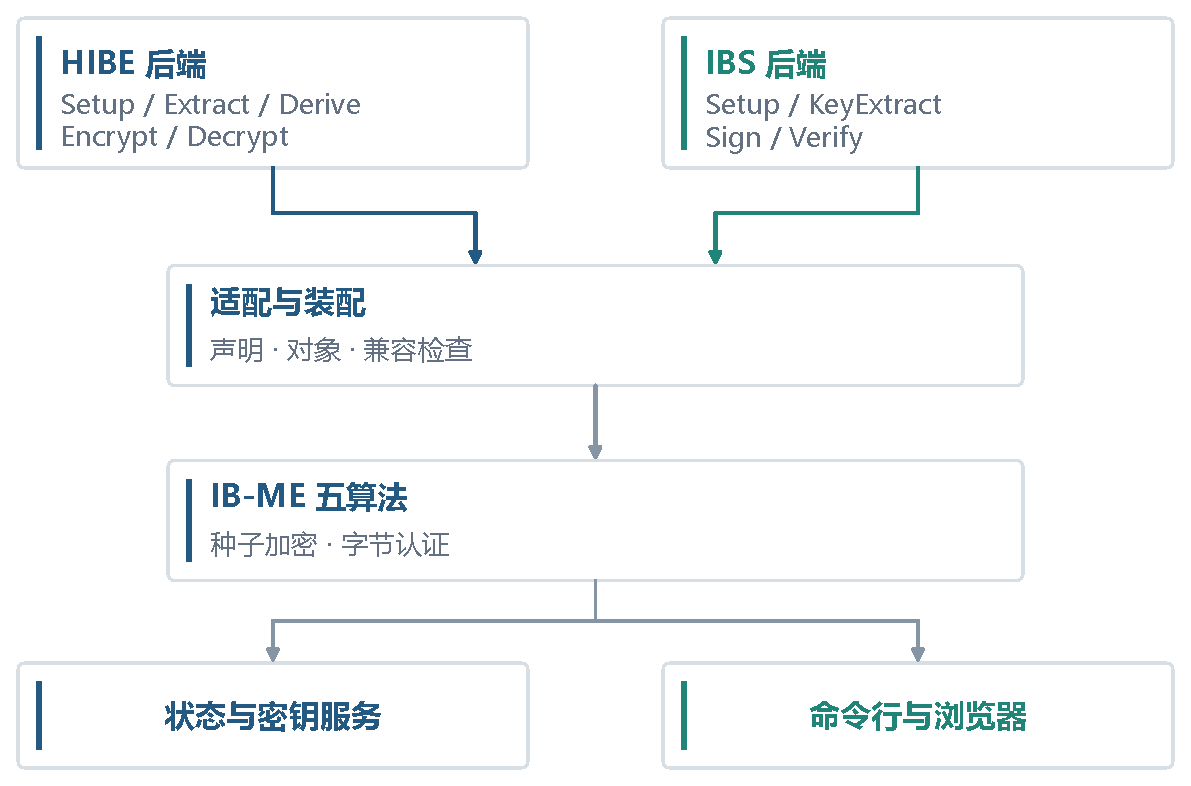
\includegraphics[width=\linewidth,height=.62\textheight,keepaspectratio]{figures/fig-03-01-architecture.pdf}
\caption{通用IB-ME系统的分层架构}
\label{fig:common-architecture}
\end{figure}

\subsection{原语接口与兼容性检查}

HIBE后端提供$\mathsf{Setup}$、$\mathsf{Extract}$、$\mathsf{Derive}$、$\mathsf{Encrypt}$和
$\mathsf{Decrypt}$；IBS后端提供$\mathsf{Setup}$、$\mathsf{KeyExtract}$、$\mathsf{Sign}$和
$\mathsf{Verify}$。每个后端还要提供公钥对象、秘密对象和密文／签名对象的规范编码与加载方法。

能力声明描述身份字节上限、HIBE明文长度、IBS签名输入上限、签名长度上界、对象编码版本以及
是否支持持久化。装配层在Setup前完成以下检查：

\begin{enumerate}
  \item 两层HIBE能够接收规范化后的接收身份与发送身份；
  \item HIBE能够加密固定的32字节种子；
  \item IBS能够签署包含接收身份、应用消息和一次性公钥承诺的规范字节；
  \item 对称加密内容的长度上限足以容纳IBS签名、消息和格式字段；
  \item 两个后端的对象版本、随机源要求和保存能力满足组合配置。
\end{enumerate}

检查结果给出应用消息上限及配置兼容性；通过检查后执行系统建立。

\section{参与方、密钥与身份顺序}

系统包含可信发钥机构、发送方和接收方。发钥机构保管HIBE与IBS的主私钥，并发布两套主公钥。公开参数$pp$描述模数、环、维数和采样参数等算法配置，并随组合配置保存。
发送者领取与自身身份$s$绑定的签名密钥，并在加密时指定接收身份$r$；接收者领取身份$r'$的
HIBE一级密钥，并在解密时填写认可发送身份$s'$。

HIBE路径固定为$(r,s)$，即第一层为接收者，第二层为发送者。接收者持有一级密钥
$\mathsf{dk}_{r'}$，再根据$s'$派生叶密钥$\mathsf{dk}_{r',s'}$。这一顺序贯穿对象编码、状态文件、签名输入和身份错配测试。

表~\ref{tab:notations}列出公共协议符号。HIBE与IBS分别维护自己的参数和对象，独立配置模数、维度与环结构；公共层保存带类型标识的对象及其规范字节。

\begin{table}[H]
\centering\small
\caption{通用协议主要符号}
\label{tab:notations}
\begin{tabularx}{\textwidth}{@{}p{.23\textwidth}X@{}}
\toprule
\rowcolor{black!8} 符号 & 含义 \\
\midrule
$r,s$；$r',s'$ & 密文指定的接收者与实际发送者；接收方密钥身份与接收者认可的发送者 \\
$\mathcal H,\mathcal S$ & 两层匿名HIBE后端与IBS后端 \\
$pp$ & 模数、环、维数及采样参数等公开算法配置 \\
$\mathsf{hpk},\mathsf{hmsk}$ & HIBE主公钥与主私钥 \\
$\mathsf{ipk},\mathsf{imsk}$ & IBS主公钥与主私钥 \\
$\mathsf{dk}_r,\mathsf{sk}_s$ & 接收者一级密钥与发送者签名密钥 \\
$M,\sigma$ & 应用消息与IBS签名 \\
$z,K$ & 32字节随机种子与由其派生的对称密钥 \\
$C_0,C_1$ & HIBE种子密文与AES-GCM载荷密文 \\
$\mathsf{ovk},\mathsf{osk},\tau$ & 一次性验签公钥、一次性签名私钥与外层签名 \\
$\mathrm{LP}(x)$ & 4字节长度前缀与字节串$x$的拼接 \\
\bottomrule
\end{tabularx}
\end{table}

系统主公钥$\mathsf{MPK}$包含$\mathsf{hpk}$、$\mathsf{ipk}$和组合配置$\mathsf{suite}$；主私钥$\mathsf{MSK}$包含$\mathsf{hmsk}$与$\mathsf{imsk}$。发钥服务另保存已发身份记录；主私钥及其发钥记录共同构成机构状态。发送方密钥$\mathsf{EK}_s$绑定
身份$s$和IBS用户密钥，接收方密钥$\mathsf{DK}_r$绑定身份$r$和HIBE一级密钥。所有对象都记录
同一组合标识、参数摘要和编码版本\addedfigref{fig:message-sequence-added}。


\begin{figure}[!htbp]
\centering
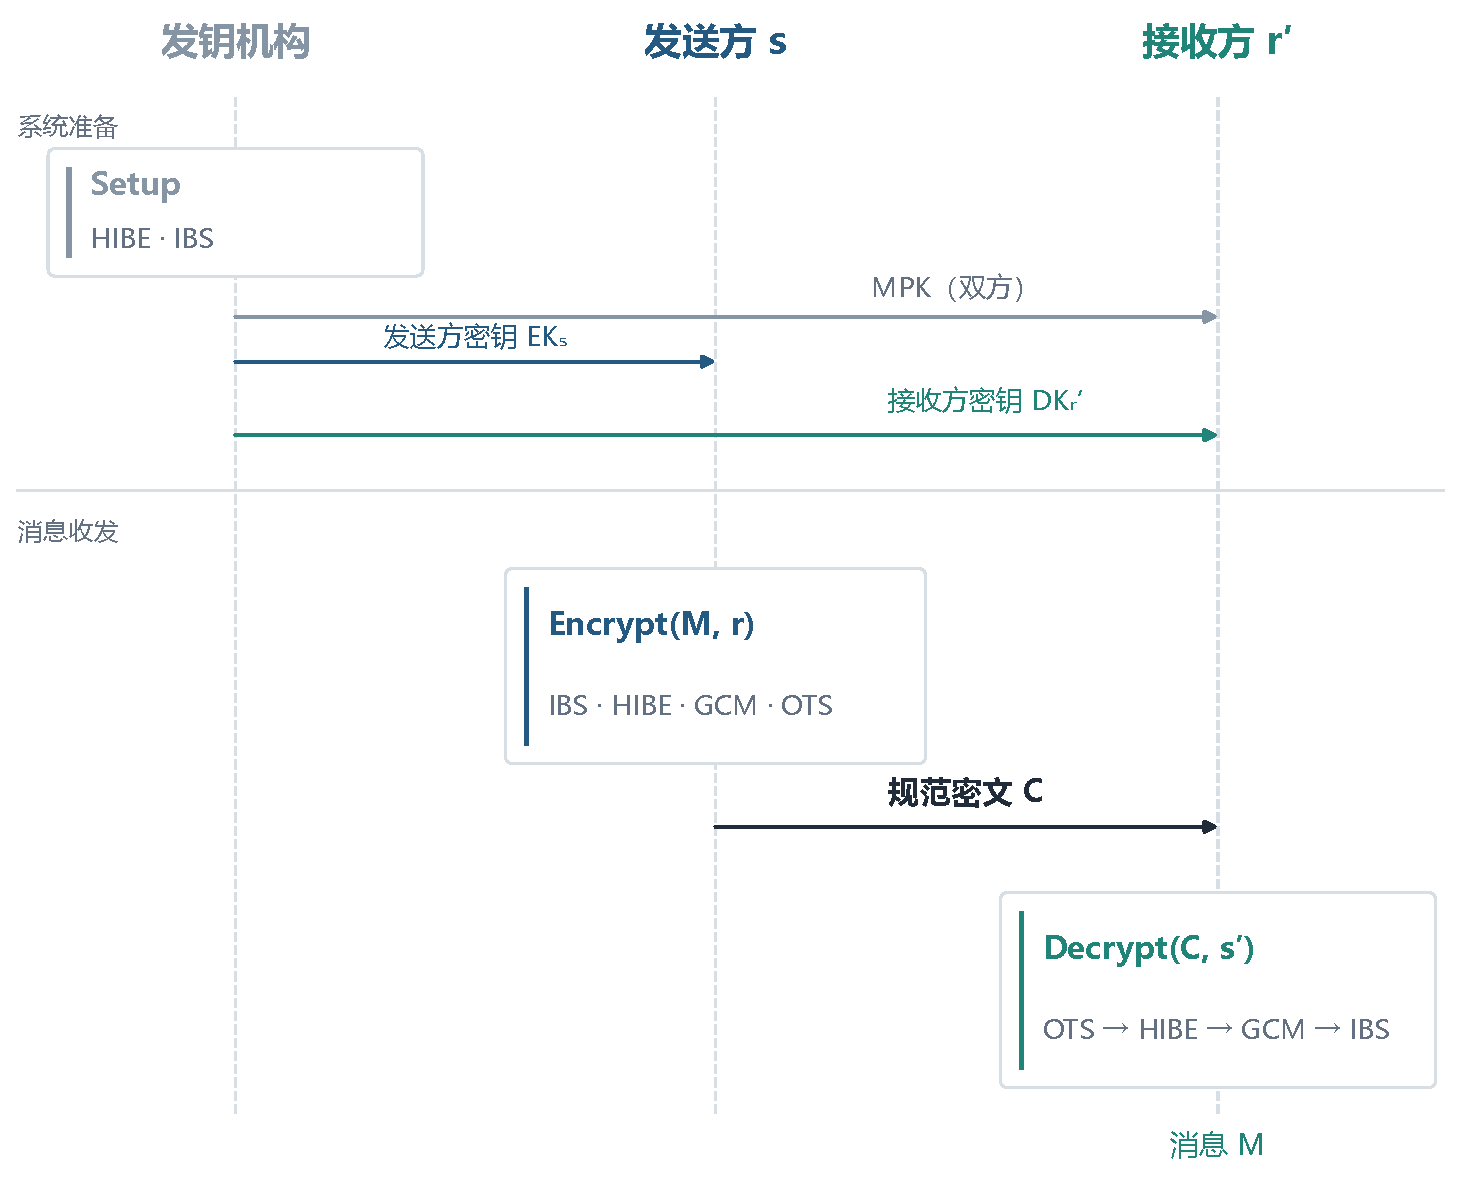
\includegraphics[width=\linewidth,height=.62\textheight,keepaspectratio]{figures/new-01-message-sequence.pdf}
\caption{系统准备与完整消息收发时序}
\label{fig:message-sequence-added}
\end{figure}

\section{IB-ME五算法伪代码}

以下五个算法给出公共协议的输入、输出、调用顺序和拒绝条件，具体后端算法见第四章。

\begin{ibmealgorithm}{系统建立 $\mathsf{Setup}$}
\label{alg:setup}
\textbf{输入：}组合配置$\mathsf{suite}$，密码随机源。\par
\textbf{输出：}主公钥$\mathsf{MPK}$，主私钥$\mathsf{MSK}$。
\begin{enumerate}
  \item 读取HIBE与IBS能力声明，执行身份、容量、编码和持久化兼容性检查；
  \item 运行$(\mathsf{hpk},\mathsf{hmsk})\leftarrow\mathcal H.\mathsf{Setup}()$；
  \item 运行$(\mathsf{ipk},\mathsf{imsk})\leftarrow\mathcal S.\mathsf{Setup}()$；
  \item 计算两套主公钥、所用参数和$\mathsf{suite}$的规范摘要；
  \item 输出$\mathsf{MPK}=(\mathsf{hpk},\mathsf{ipk},\mathsf{suite})$及由机构保存的
        $\mathsf{MSK}=(\mathsf{hmsk},\mathsf{imsk},\mathsf{suite})$。
\end{enumerate}
\end{ibmealgorithm}

\begin{ibmealgorithm}{发送方密钥生成 $\mathsf{SenderKeyGen}$}
\label{alg:sender-keygen}
\textbf{输入：}$\mathsf{MSK}$，发送身份$s$。\par
\textbf{输出：}发送方密钥$\mathsf{EK}_s$或拒绝$\bot$。
\begin{enumerate}
  \item 按发送者域标识和长度前缀规范编码$s$，检查身份长度；
  \item 调用$\mathsf{sk}_s\leftarrow\mathcal S.\mathsf{KeyExtract}(\mathsf{imsk},s)$；
  \item 检查返回对象类型、参数摘要和身份绑定；
  \item 输出$\mathsf{EK}_s=(s,\mathsf{sk}_s,\mathsf{suite})$，并由固定发钥服务记录摘要。
\end{enumerate}
\end{ibmealgorithm}

\begin{ibmealgorithm}{接收方密钥生成 $\mathsf{ReceiverKeyGen}$}
\label{alg:receiver-keygen}
\textbf{输入：}$\mathsf{MSK}$，接收身份$r$。\par
\textbf{输出：}接收方密钥$\mathsf{DK}_r$或拒绝$\bot$。
\begin{enumerate}
  \item 按接收者域标识和长度前缀规范编码$r$，检查身份长度；
  \item 调用$\mathsf{dk}_r\leftarrow\mathcal H.\mathsf{Extract}(\mathsf{hmsk},r)$；
  \item 检查一级密钥的参数摘要、层级和身份绑定；
  \item 输出$\mathsf{DK}_r=(r,\mathsf{dk}_r,\mathsf{suite})$。
\end{enumerate}
\end{ibmealgorithm}

\begin{ibmealgorithm}{消息加密 $\mathsf{Encrypt}$}
\label{alg:encrypt}
\textbf{输入：}$\mathsf{MPK}$，$\mathsf{EK}_s$，接收身份$r$，消息$M$。\par
\textbf{输出：}规范密文$C$或拒绝$\bot$。
\begin{enumerate}
  \item 检查组合摘要、身份和消息上限，生成一次性密钥对$(\mathsf{ovk},\mathsf{osk})$；
  \item 计算$d_{\rm ovk}=H_{\rm commit}(\mathsf{ovk})$，将$M$和$d_{\rm ovk}$编码为内部消息结构$E$，
        再令$E_{\rm sig}=\operatorname{EncMsg}(r,E)$；
  \item 生成$\sigma\leftarrow\mathcal S.\mathsf{Sign}(\mathsf{sk}_s,E_{\rm sig})$，编码内部载荷$P$；
  \item 新取32字节种子$z$，调用$C_0\leftarrow\mathcal H.\mathsf{Encrypt}
        (\mathsf{hpk},(r,s),z)$；
  \item 由$z$派生$K$，使用AES-256-GCM加密$P$得到$C_1$；
  \item 对公开上下文、$\mathsf{ovk}$、$C_0$和$C_1$的规范字节生成一次性签名$\tau$；
  \item 输出$C=\operatorname{Encode}(\mathsf{ctx},\mathsf{ovk},C_0,C_1,\tau)$。
\end{enumerate}
\end{ibmealgorithm}

\begin{ibmealgorithm}{匹配解密 $\mathsf{Decrypt}$}
\label{alg:decrypt}
\textbf{输入：}$\mathsf{MPK}$，$\mathsf{DK}_{r'}$，认可发送身份$s'$，密文$C$。\par
\textbf{输出：}消息$M$或拒绝$\bot$。
\begin{enumerate}
  \item 规范解析$C$，检查版本、字段长度、配置摘要和公开上下文；
  \item 用$\mathsf{ovk}$验证$\tau$；失败则返回$\bot$；
  \item 计算$\mathsf{dk}_{r',s'}\leftarrow\mathcal H.\mathsf{Derive}(\mathsf{dk}_{r'},s')$；
  \item 解开$C_0$得到$z$，派生$K$并验证GCM标签，恢复$P$；
  \item 解析$E$与$\sigma$，计算$E_{\rm sig}=\operatorname{EncMsg}(r',E)$，以身份$s'$调用
        $\mathcal S.\mathsf{Verify}$；
  \item 解析$E$中的$d_{\rm ovk}$与$M$，核对$d_{\rm ovk}$来自外层$\mathsf{ovk}$；
  \item 所有检查通过后返回$M$；任一步失败均返回$\bot$。
\end{enumerate}
\end{ibmealgorithm}

\section{基于短种子封装的混合加密}

IBS签名尺寸从数KiB到数MiB不等，而HIBE直接明文容量通常只有几十字节。公共协议采用
KEM--DEM式混合结构：HIBE加密固定的32字节随机种子，对称加密承担签名和应用消息组成的
可变长度载荷。

身份编码先写入域标识、发送或接收角色、身份的实际长度和身份字节，再在末尾填入0字节，
使身份部分达到规定长度。长度字段用于恢复原始身份，发送者与接收者使用不同角色标识。
当前身份上限为64字节，加入这些字段后，内部身份固定为86字节。HIBE封装和密钥派生为
\begin{align*}
 C_0&\leftarrow\mathcal H.\mathsf{Encrypt}
       (\mathsf{hpk},(\operatorname{Pad}_P(r),\operatorname{Pad}_C(s)),z),\\
 K&\leftarrow\operatorname{HKDF\text{-}SHA256}(z;\mathsf{ctx}_H,\mathsf D_{\rm kdf}),\\
 C_1&\leftarrow\operatorname{AES\text{-}256\text{-}GCM.Enc}(K,n,P;\mathsf{AAD}).
\end{align*}
这里$n$是每条消息新生成的12字节随机数（nonce）。HKDF和GCM分别采用RFC~5869与NIST SP~800-38D规定
的原语\cite{rfc5869,nist2007gcm}。附加认证数据包含组合上下文、HIBE种子密文$C_0$、nonce和载荷
长度。修改种子密文或把对称密文移动到另一组合中，都会导致认证失败。

混合结构把底层HIBE需要处理的明文固定为32字节。对称加密内容包含IBS签名、应用消息和格式字段，
组合配置为这部分内容设置总长度上限。装配层结合IBS的签名输入上限和最大签名长度，扣除签名及
格式字段所占空间，在建立主密钥前计算应用消息可用的字节数。

\section{发送身份绑定与完整密文字节认证}

完整密文认证覆盖传输版本、字段边界、HIBE种子密文和对称密文。本作品使用Lamport型一次性
签名连接内外两层认证\cite{lamport1979ots}。加密时先把一次性验签公钥承诺写入IBS签名消息：
\begin{align*}
 d_{\rm ovk}&=H_{\rm commit}(\mathsf{ovk}),\\
 E&=\mathsf D_{\rm bound}\parallel\mathrm{LP}(d_{\rm ovk})
       \parallel\mathrm{LP}(M),\\
 E_{\rm sig}&=\operatorname{EncMsg}(r,E),\\
 \sigma&\leftarrow\mathcal S.\mathsf{Sign}
       (\mathsf{sk}_s,E_{\rm sig}),\\
 P&=\mathsf D_{\rm sig}\parallel\mathrm{LP}(\sigma)\parallel\mathrm{LP}(E).
\end{align*}
得到HIBE种子密文和对称密文后，再对全部内层传输字节签名：
\[
 \tau\leftarrow\mathsf{OTS.Sign}_{\mathsf{osk}}
    (\mathsf D_{\rm ct}\parallel\mathrm{LP}(\mathsf{ctx})
      \parallel\mathrm{LP}(\mathsf{ovk})\parallel\mathrm{LP}(C_0,C_1)).
\]

接收端先验证外层一次性签名，再解密载荷并检查IBS签名中的$d_{\rm ovk}$。攻击者即使重新生成
一次性密钥并为修改后的外层字节签名，也不能让原IBS签名承诺新的公钥；原一次性签名也不能验证
任何变化后的种子密文或对称密文\addedfigref{fig:ciphertext-layout-added}。

\begin{figure}[!htbp]
\centering
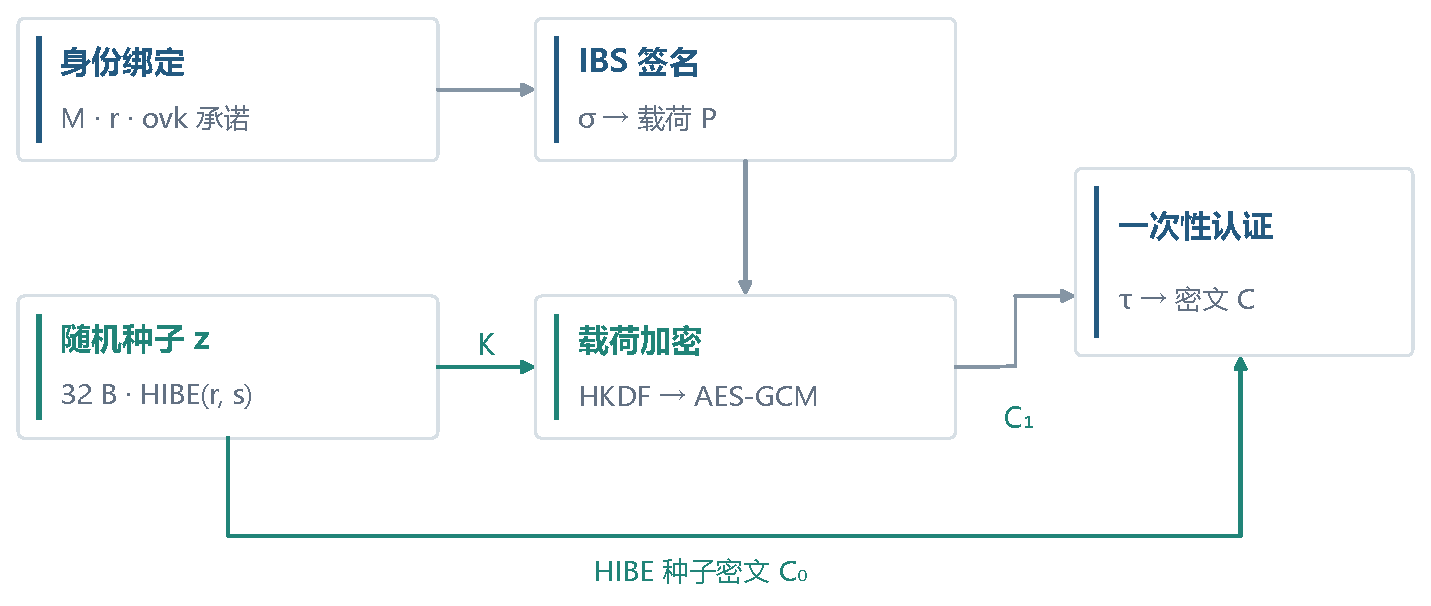
\includegraphics[width=\linewidth,height=.62\textheight,keepaspectratio]{figures/fig-03-02-encryption.pdf}
\caption{身份签名、短种子封装与完整字节认证的关系}
\label{fig:protocol-generation}
\end{figure}


\begin{figure}[!htbp]
\centering
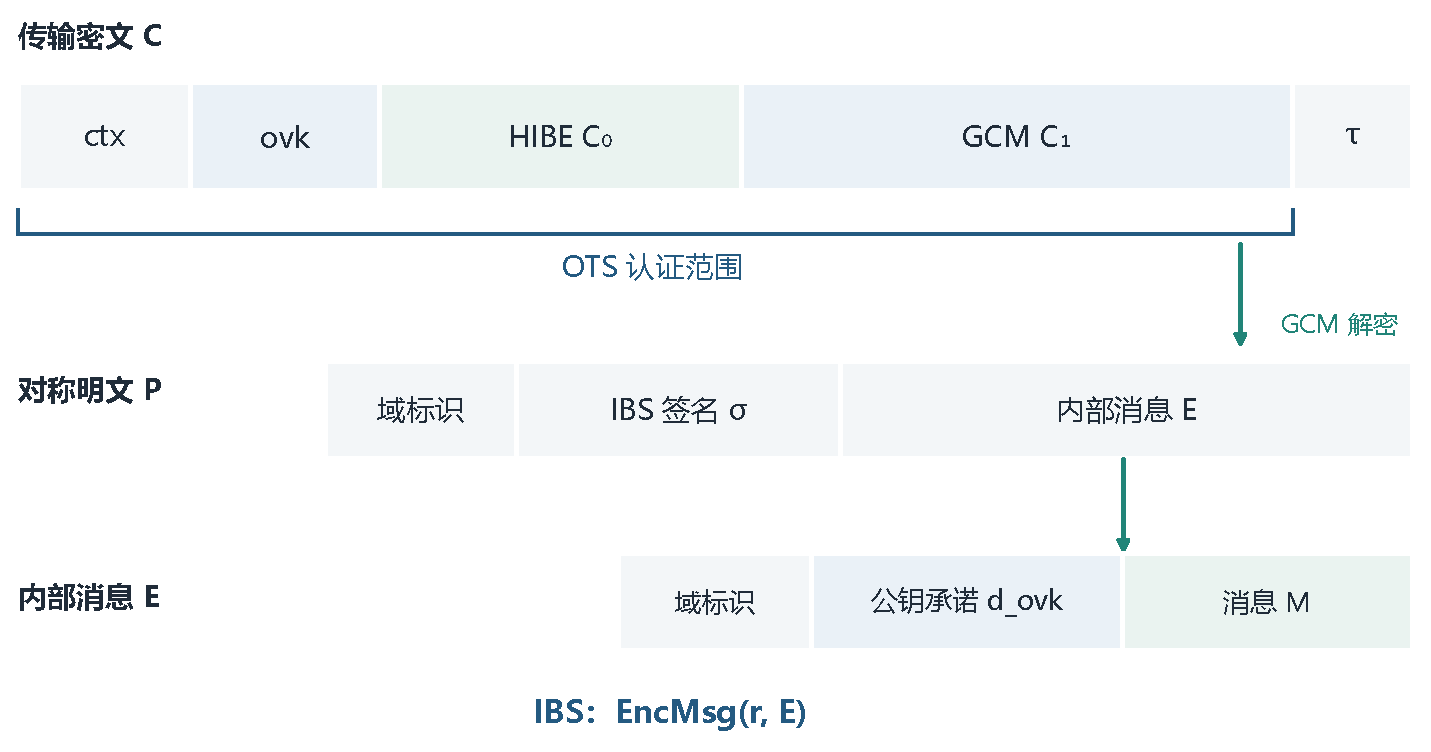
\includegraphics[width=\linewidth,height=.62\textheight,keepaspectratio]{figures/new-02-ciphertext-layout.pdf}
\caption{密文层次与两层签名的认证范围}
\label{fig:ciphertext-layout-added}
\end{figure}

\section{规范编码、状态与异常处理}

\subsection{规范对象编码与状态恢复}

所有公钥对象、机构状态、角色密钥和密文均使用类型标识、版本、参数摘要和长度前缀。编码器固定字段
顺序，解码器检查总长度、字段上限、未知或重复字段、整数范围和末尾未使用位。解码后重新编码必须
得到相同字节，从而避免同一数学对象存在多种可接受表示。

长期状态包括主私钥、已发身份记录、发送者密钥和接收者一级密钥；会话状态只保存某次固定身份对
的叶密钥和上下文；逐消息对象包括随机种子、GCM nonce、一次性签名密钥和密文。三类状态采用
不同生命周期，逐消息随机量不得写入固定发钥记录，会话叶密钥也不作为长期角色密钥导出。

恢复对象时，程序先加载公开配置，再检查对象中的算法名、参数摘要和身份绑定。恢复过程加载已有身份密钥及其绑定信息。这样，命令行和浏览器入口可以在不同进程中使用同一套已生成状态。

\subsection{正确性与异常处理}

当$r=r'$且$s=s'$时，接收端派生的叶密钥与加密路径一致，HIBE恢复同一个$z$；HKDF得到同一
$K$，GCM恢复载荷$P$；IBS以同一发送身份验证签名，内外一次性公钥承诺也一致，最终输出$M$。

接收身份错误时，一级密钥不能形成正确叶密钥；认可发送身份错误时，HIBE第二层路径和IBS验签
身份同时改变。应用消息、IBS签名或一次性公钥承诺变化时，IBS验证失败；种子密文、对称密文、上下文、
nonce或外层签名变化时，一次性签名或GCM验证失败。

解码器先检查魔数、版本、总长度和字段上限，再分配大型对象。未知字段、重复字段、截断、追加、
非规范整数、错误对象类型和配置摘要不匹配均直接拒绝。依赖缺失和资源不足返回运行错误；身份错配与认证失败返回协议拒绝。

\subsection{本章小结}

本章给出了与具体格方案无关的IB-ME公共协议。五算法伪代码明确了原语调用和拒绝顺序；短种子
封装解决HIBE明文容量与大签名之间的矛盾；IBS和一次性签名分别绑定发送身份与完整密文字节；
规范对象和状态边界支持固定发钥与重启恢复。由此，不同后端可以共享同一身份语义、处理顺序和
失败结果。
